\documentclass[10pt]{usetex-v1}
%\documentclass[10pt,workingdraft]{usetex-v1}

\usepackage{epsfig}
\usepackage{url}
\usepackage{times}
%\usepackage{subfigure}
\usepackage{tabularx}
%\usepackage{scalefnt}
%\usepackage{endnotes}
%\usepackage{footnote}
%\usepackage{multirow}
%\usepackage{amsmath}
%\usepackage{amssymb}
%\usepackage{booktabs}
%\usepackage{listings}
\usepackage{vmargin}
\usepackage{cite}
\usepackage{alltt}
%\usepackage{psfrag}
%\usepackage{boxedminipage}
\usepackage{colortbl}
\usepackage{xspace}
%\usepackage[showframe=true]{geometry}
\usepackage{enumitem}
%\usepackage{program}
\usepackage{listings}

%\numberwithin{equation}{section}
% space b/t list \item's
\newcommand{\smallitemsep}      {\setlength{\itemsep}{-0.5ex}}
%\newcommand{\smallitemsep}     {}

\newcommand{\stt}[1]            {\texttt{\small #1}}

% space b/t captions and their floats
\newcommand{\captionsep}        {\vspace{-1.00em}}
\newcommand{\tabcaptionsep}     {\vspace{-0.50em}}
%\newcommand{\captionsep}       {}
% size of caption font
%\newcommand{\captionfont}      \tiny
\newcommand{\captionfont}       \itshape
\newcommand{\capfont}           \small
%\newcommand{\capfont}          {}

\newcommand{\etal}{\emph{et al.}}

% make tables narrower in width so they fit better in twocolumn formats
\addtolength{\tabcolsep}{-0.5\tabcolsep}
% less space between rows of tables
\renewcommand{\arraystretch}{0.95}
%% space between columns in twocolumn mode
%\addtolength{\columnsep}{-0.1\columnsep}

\newenvironment{consistifyoff}[0]{}      {}

\newenvironment{ezbox}[1]%
{
 \footnotesize
 \begin{center}
 \begin{boxedminipage}[t]{#1}
 \begin{alltt}
}
{
 \end{alltt}
 \end{boxedminipage}
 \end{center}
}

\newenvironment{smalltt}%
{
\vspace{-0.5em}
\footnotesize
\begin{alltt}
}
{
\end{alltt}
\vspace{-0.5em}
}

%\lstset{language=C, basicstyle=\ttfamily\small}
\hyphenation{vnode}

% redefine \url font to normal font
\def\UrlFont{\sl\footnotesize}

\begin{document}

\title{Social Networks: Identify Important Nodes In Ego Network}

\author{
    \authname{Arvind Chaudhary and Bharat Singh}
    \authaddr{Stony Brook University}
}

\setpapersize{USletter}
% % \setmarginsrb{leftmargin}{topmargin}{rightmargin}{bottommargin}%
% %    {headheight}{headsep}{footheight}{footskip}
\setmarginsrb{25mm}{25mm}{25mm}{15mm}{0mm}{0mm}{10mm}{10mm}

\pagestyle{plain}

%\newcommand{\stt}[1]                    {\texttt{\small #1}}
%\def\gtilda{\kern -.15em\lower .7ex\hbox{\~{}}\kern .04em}

%%%%%%%%%%%%%%%%%%%%%%%%%%%%%%%%%%%%%%%%%%%%%%%%%%%%%%%%%%%%%%%%%%%%%%%%%%%%%%
%%% SQUEEZE SOME SPACES
%\addtolength{\parskip}{4.5\parskip}
%\setlength{\partopsep}{0mm}
%\setlength{\topsep}{0mm}
%\addtolength{\baselineskip}{-0.03\baselineskip}
%\setlength{\parskip}{-0.5ex}
%\renewcommand{\baselinestretch}{0.9}
%\addtolength{\tabcolsep}{-0.5\tabcolsep}
%\setlength{\topsep}{-2.0ex}
%
%% make tables narrower in width so they fit better in twocolumn formats
%\addtolength{\tabcolsep}{-0.4\tabcolsep}
%% less space between rows of tables
%\renewcommand{\arraystretch}{0.95}
%% allow up to 4 floats at top of page (default=2)
\setcounter{topnumber}{4}
\setcounter{dbltopnumber}{8}	% for double-floats
%% allow up to 2 floats at bottom of page (default=1)
\setcounter{bottomnumber}{2}
%% allow up to 8 floats total per page (default=3)
\setcounter{totalnumber}{8}

% %% less space above/below floats that are at top/bottom of pages
\addtolength{\floatsep}{-0.5\floatsep}
\addtolength{\dblfloatsep}{-0.5\dblfloatsep}
% %% less space above/below "h" floats that are in the middle of text
\addtolength{\intextsep}{-0.5\intextsep}
\addtolength{\textfloatsep}{-0.5\textfloatsep}
\addtolength{\dbltextfloatsep}{-0.5\dbltextfloatsep}
% smaller space around captions
\addtolength{\abovecaptionskip}{-0.75\abovecaptionskip}

%% Control floats
\renewcommand{\topfraction}{1.0} % max percentage a float can take at top
\renewcommand{\bottomfraction}{1.0} % max percentage float can take at bottom
\renewcommand{\textfraction}{0.01} % min percentage text can take on page
%\renewcommand{\textfraction}{0.5} % min percentage text can take on page
\renewcommand{\floatpagefraction}{0.99} % min fraction of float page used
\renewcommand{\dblfloatpagefraction}{0.99} % min fraction of float page used

%% space between columns in twocolumn mode
%\addtolength{\columnsep}{-0.1\columnsep}
%% width of text on a page
%\addtolength{\textwidth}{0.01\textwidth}

%%%%%%%%%%%%%%%%%%%%%%%%%%%%%%%%%%%%%%%%%%%%%%%%%%%%%%%%%%%%%%%%%%%%%%%%%%%%%%

%\tableofcontents
\maketitle

\begin{abstract}

% dummy entry to force emacs not to indent abstract text
\vspace{0mm}

%"sales pitch".  a short 1-2 pgfs, few sentences,
%to convince the reader to read the rest.
%
%1. there's a problem
%
%2. what others have done about it (WHY no good)
%
%3. what you did (WHY it's better)
%
%4. WHY your stuff is better (some results?)
%
%No citations.

This projects aims to identify different social foci in an ego network
of facebook friends.  Social foci in a group will be one of the most
important node in that particular group.

We have used various methods to measure the importance of a node
such as betweenness centrality, closeness centrality and eigenvector
centrality.  We also plan to divide the graph into different clusters
using k­means clustering and then report centroid of each cluster as
foci for respective cluster.

Keywords: k­means clustering, betweenness, closeness, eigenvector.
\end{abstract}

%%%%%%%%%%%%%%%%%%%%%%%%%%%%%%%%%%%%%%%%%%%%%%%%%%%%%%%%%%%%%%%%%%%%%%%%%%%%%%
%% For Emacs:
% Local variables:
% fill-column: 70
% End:
%%%%%%%%%%%%%%%%%%%%%%%%%%%%%%%%%%%%%%%%%%%%%%%%%%%%%%%%%%%%%%%%%%%%%%%%%%%%%%
%% For Vim:
% vim:textwidth=70
%%%%%%%%%%%%%%%%%%%%%%%%%%%%%%%%%%%%%%%%%%%%%%%%%%%%%%%%%%%%%%%%%%%%%%%%%%%%%%
% LocalWords: eCryptfs, POSIX, UID

\section{Introduction}
\label{intro}

eCryptfs~\cite{halcrow2007ecryptfs} is a POSIX-compliant
enterprise-class stacked cryptographic file system for Linux.  It is
derived from Erez Zadok's Cryptfs~\cite{zadok:cryptfs}, implemented
through the FiST framework for generating stacked file systems.
eCryptfs is a native Linux file system.  It builds as a stand-alone
kernel module for the Linux kernel; there is no need to apply any
kernel patches.  It is available in the mainline Linux Kernel as of
2.6.19.  eCryptfs is widely used, as the basis for Ubuntu's Encrypted
Home Directory, natively within Google's ChromeOS, and transparently
embedded in several network attached storage (NAS) devices.

eCryptfs stores cryptographic meta data in the header of each file, so
that encrypted files can be copied between hosts.  The file will be
decrypted only if a valid key is produced.  There is no need to keep
track of any additional information aside from what is already in the
encrypted file itself.

eCryptfs simply requires that a File Encryption Key (FEK) be
associated with any given inode in order to decrypt the contents of
the file on disk.  This prevents an attacker from accessing the file
contents outside the context of the trusted host environment.  For
instance, storage media is lost or stolen.  This is the only type of
unauthorized access that eCryptfs is intended to prevent.

But in a multiuser environment, once a user have access to the
encrypted data, there is no prevention from another user accessing the
data even if that user does not have valid key.  To tackle this
problem there are many access control mechanisms, but it is very
difficult to deny access to a root user via access control mechanisms.
Thus all the users with sudo permission can also access the data that
a user does not want to share.  eCryptfs offers no additional access
control functions other than what is already implemented via standard
POSIX file permissions, access control mechanisms (capabilities, SE
Linux) and so forth.

We have introduced a policy based authentication mechanism inside
eCryptfs.  It is an additional check to prevent unauthorized users
inside a trusted host environment from accessing the encrypted data,
even root user is not allowed.  Based on our experimental results we
see that this mechanism does not add much overhead in the current
performance of eCryptfs.

%Typical length: 1-1.5 pages.

%Intro text with a citation~\cite{cryptfs}.

%one-page summary of entire paper: - same 4 steps as abstract, but 1
%pgf each, instead of 1 sentence.  - intro very important: most
%reviewers make up their mind early on.
%
%When to write intro: - last: to ensure it properly summarizes entire
%paper.  - first: useful as an outline for rest of work
%
%Often best to write an outline of whole paper/ideas.

The rest of this document is organized as follows.  Section 2
describes the background and current limitations of eCryptfs.  Section
3 describes our proposed design.  Section 4 describes evaluation plan
and results.  Section 5 describes related work.  Section 6 describes
how the solution can be extended for different other methods,
conclusion and future work.

%%%%%%%%%%%%%%%%%%%%%%%%%%%%%%%%%%%%%%%%%%%%%%%%%%%%%%%%%%%%%%%%%%%%%
%% For Emacs:
% Local variables:
% fill-column: 70
% End:
%%%%%%%%%%%%%%%%%%%%%%%%%%%%%%%%%%%%%%%%%%%%%%%%%%%%%%%%%%%%%%%%%%%%%
%% For Vim:
% vim:textwidth=70
%%%%%%%%%%%%%%%%%%%%%%%%%%%%%%%%%%%%%%%%%%%%%%%%%%%%%%%%%%%%%%%%%%%%%%
% LocalWords:

%\section{Background}
\label{bg}

%Background...
%
%Typical length: 0 pages to 1.0.
%
%Background and Related Work can be similar.  Most citations will be
%in this section.
%
%1. Describe past work and criticize it, fairly.  Use citations to
%JUSTIFY your criticism!  Problem: hard to compare to YOUR work, b/c
%you've not yet described your work in enough detail.  Solution: move
%this text to Related Work at end of paper.
%
%2. Describe in some detail, background material necessary to
%understand the rest of the paper.  Doesn't happen often, esp. if
%you've covered it in Intro.
%
%Example, submit a paper to a storage conference: reviewers are
%experts in storage.  Don't need to tell them about basic disk
%operation.  But if your paper, say, is an improvement over an
%already-advanced data structure (eg., COLA), then it'd make sense to
%describe basic COLA algorithms in some detail.
%
%Important: open the bg section with some "intro" text to tell reader
%what to expect (so experienced readers can skip it).
%
%If your bg material is too short, can fold it into opening of
%'design' section.

eCryptfs protects data confidentiality even when an unauthorized agent
gains access to the host machine.  A secret paraphrase is used to
control access to the file contents.  Properties like file name, size
and other associated meta-data are left unencrypted.  Crypto
information for each file is stored as crypt header following the
rfc2240~\cite{rfc2240} format  along with eCryptfs marker in the file
itself, so files are portable in the event of a system or disk
failure.  Even host and persistent storage is not trusted here.

\paragraph{Current Limitations}
\begin{itemize}
\item Any user can decrypt the file, if a valid key is produced.  Once
	the file is decrypted, anyone on that host can read or write
	based on Unix permissions.  Such behavior is not suitable for
	a multi-user or file sharing environment.
\item Anyone with file permissions can delete the file.  Even if the
	file is encrypted any user with Unix permissions can modify
	the file, it may corrupt the crypto headers, hence the file
	cannot be decrypted.
\item Access revocation does not work without unmounting the eCryptfs
	file system, making it a disruptive operation.
\item There is no support for key expiry in eCryptfs.  eCryptfs can
	leverage the key expiration feature of Linux
	kernel~\cite{keyexpire}.
\end{itemize}

%%%%%%%%%%%%%%%%%%%%%%%%%%%%%%%%%%%%%%%%%%%%%%%%%%%%%%%%%%%%%%%%%%%%%%%%%%%%%%
%% For Emacs:
% Local variables:
% fill-column: 70
% End:
%%%%%%%%%%%%%%%%%%%%%%%%%%%%%%%%%%%%%%%%%%%%%%%%%%%%%%%%%%%%%%%%%%%%%%%%%%%%%%
%% For Vim:
% vim:textwidth=70
%%%%%%%%%%%%%%%%%%%%%%%%%%%%%%%%%%%%%%%%%%%%%%%%%%%%%%%%%%%%%%%%%%%%%%%%%%%%%%
% LocalWords:

%\section{Design}
\label{Design}

%Opening text...  Typical length: 3-5 pages.
%
%Hardest section to write.  A lot of possible interdependencies.
%
%If you find that you have to have a ``forward'' reference to a
%section of text you've not described yet, it usually means that the
%structure of your paper is wrong.  So avoid fwd refs.  Backward
%references to previous sections is ok, as long as it's not too far in
%the beginning of the paper.
%
%Do an outline of design even print a Table of Contents
%
%Opening: tell reader what to expect.
%
%Open with key design goals, in descending importance.
%
%General rule: whenever you LIST 2 or more items, THINK about their
%order (should it be importance order? chronological?  categorical?)
%
%(A) What are your design goals, and what do they get you?  Separate
%goals with HOW you achieve them.  Possible goals can include:
%
%- improved performance
%
%- improved scalability (same as perf.  but need to test "multiple"
%machines)
%
%- better energy consumption
%
%- improved security (hard to prove "better" security)
%
%- versatility: has more functionality that can be utilized in more
%settings.  A generalization of past specific work.
%
%- compatibility: works with many existing systems, possibly
%unmodified (or with few modifications).
%
%- other design goals?
%
%(B) briefly describe HOW you would accomplish each of your design
%goals.
%
%(C) Show a high-level architectural figure whole system, and describe
%every "box" of section of the figure.
%
%Start with high-level detail of each components, then go into greater
%detail.
%
%(D) Bulk of design: go over every design goal and architectural
%component, and describe it in detail.
%
%Key: don't just say WHAT you did, but WHY you did that.  WHY, WHY,
%WHY!
%
%Tense: past tense for what was designed, present tense to describe
%system operation.  Switch b/t past and present consistently.  NO
%future tense!
%
%-----------------------------------------------------------------------------

\subsection{Centrality}
Various indicators of centrality identify the most important vertices
within a graph.  Most commonly used indicators of centrality are:
\begin{itemize}[leftmargin=*]
\item
Closeness Centrality
\item
Betweenness Centrality
\item
Eigenvector Centrality
\end{itemize}

\paragraph{Closeness Centrality}
Closeness centrality denotes how close a nodes is with different
nodes in the graph.  Central nodes are important, as they can reach
the whole network more quickly than non-central nodes.


\paragraph{Betweenness Centrality}
Node betweenness counts the number of shortest paths that pass through
the node. Betweenness centrality is a measure of how influential a
node is in diffusion of information in the graph.  It is calculated as
fraction of shortest paths that pass through this node.

\paragraph{Eigenvector Centrality}
A nodes is important if it is connected to a number of important
nodes.  Eigenvector centrality denotes the numbers of important nodes
a node is connected to.  Eigenvector centrality corresponds to the
top eigenvector of the adjacency matrix.

\subsection{K-means clustering}
vide the ego network in different clusters using k-means clustering
algorithm.  The centroid of each cluster can be seen as the foci for
respective cluster.  We have used standard MATLAB k-means clustering
APIs to divide the graph into clusters.  We project the data to one
dimension space using spectral clustering technique.


%\subsection{System Operation}
%
%Example of subsection...
%
%%-----------------------------------------------------------------------------
%\paragraph{Garbage collection}
%%
%Example of a pragraph heading.
%
%\begin{figure}[htbp] \begin{centering}
%\epsfig{file=figures/lba-ind-example.eps,angle=270,width=1.00\linewidth}
%\caption{LBA indirection example.  The host first writes LBAs 23,
%352, 53, 63, 64, 65, 52, and 29.  The second write sequence is 75,
%76, 23, 52, 324, 263, and 636.  This causes LBAs 23 and 52 to become
%garbage.  Moreover, reading LBAs sequentially requires reading ABAs
%randomly.} \label{fig:lba-ind} \end{centering} \end{figure}
%
%
%Here's how you refer to Figure~\ref{fig:lba-ind}.
%
%\begin{itemize}
%
%\item itemized list item 1
%
%\item item 2
%
%\end{itemize}
%
%
%\textbf{* TENSE USE: past, present, and future}
%
%By default, everything should be written in PAST tense.  "We designed
%a system and evaluated it."
%
%Use present tense ONLY to describe system operation.  "Our system
%sends a message to the server."
%
%Use future tense ONLY in "future work" section!


%%%%%%%%%%%%%%%%%%%%%%%%%%%%%%%%%%%%%%%%%%%%%%%%%%%%%%%%%%%%%%%%%%%%%%%%%%%%%%
%% For Emacs:
% Local variables:
% fill-column: 70
% End:
%%%%%%%%%%%%%%%%%%%%%%%%%%%%%%%%%%%%%%%%%%%%%%%%%%%%%%%%%%%%%%%%%%%%%%%%%%%%%%
%% For Vim:
% vim:textwidth=70
%%%%%%%%%%%%%%%%%%%%%%%%%%%%%%%%%%%%%%%%%%%%%%%%%%%%%%%%%%%%%%%%%%%%%%%%%%%%%%
% LocalWords:

\section{Evaluation}
\label{eval}

%Evaluation section...
%
%Length: 3-4 pages (graphs take a lot of space!)
%
%Tell reader what to expect.
%
%Eval is "proof" that your design is good.
%MATCH eval goals with design goals.
%
%Eval section is easier to write, but longest one to produce
%results for.  Whereas design section has complex structure, eval
%is more 'flat'.
%
%Structure:
%
%1.  list eval goals, should match design goals
%
%2.  briefly list how you plan to prove those goals.
%
%3.  describe your testbed: h/w + s/w platform to run tests on.
%Give enough detail so it can be reproduced by ANYONE.
%
%4.  describe your benchmarks in detail:
%
%(4a) Micro benchmarks: test specific feature (e.g., read or
%write performance).  Usually u-bench are designed to highlight
%worst/best case behavior of your system.  Be to list both best
%and worst.
%
%(4b) Macro benchmarks (general purpose benchmarks): test whole
%system (e.g., run a Web server exerciser, or TPC for database).
%
%Some tests should compare YOUR system to past systems, or a
%"before and after" comparison.
%
%For every possible variable in your system, design a set of
%independent tests (re: compression study's dimensions).  Justify
%need to vary each variable (the more variables, the more
%experiments you have to run).
%
%5.  Describe your benchmarking methodology
%
%Statistical stability: how many times you run each test? do you
%compute standard deviations, half-width intervals (for student-t
%distribution), RMS, or other metric of stability?  Say how many
%times you ran each test, and what were the stability metrics.
%
%Ex."we ran every test at least 10 times, and computed the
%standard deviation as a percentage of the mean.  In all cases,
%the percentage was less than 5\%, unless otherwise noted."
%
%6.  List every benchmark result, for each test
%
%(a) a graph or table or other figure, plus caption.
%(b) followed by an explanation of the figure: say what one sees
%    in the figure, then explain WHY it is so.
%
%7.  Optional: if eval section longer than usual, end it with a
%one-paragraph summary of eval results.


\begin{figure*}[!ht]
    \centering
    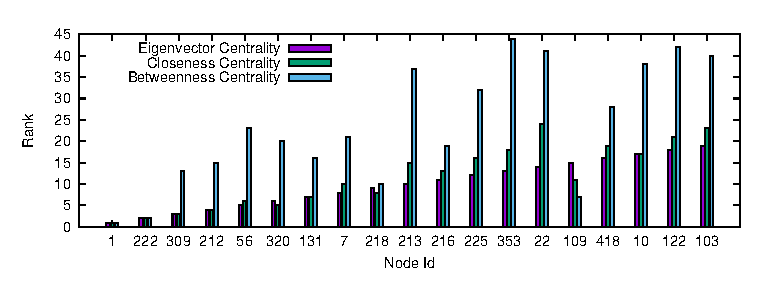
\includegraphics[width=1\textwidth]{figures/social-result_eigen.eps}
    \caption{Rank comparison for top 20 nodes ranked on eigenvector centrality with other centrality scores.}
    \label{fig:social-result-eigen}
\end{figure*}

\begin{figure*}[!ht]
    \centering
    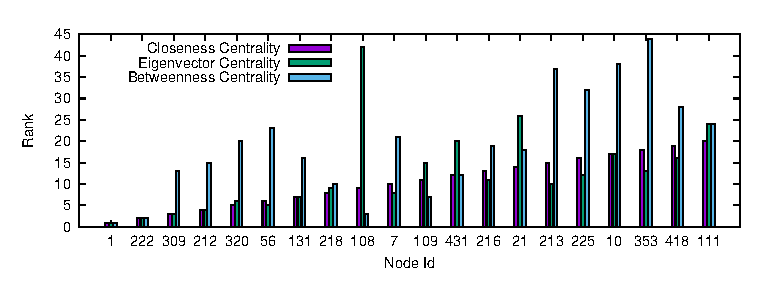
\includegraphics[width=1\textwidth]{figures/social-result_closeness.eps}
    \caption{Rank comparison for top 20 nodes ranked on closeness centrality with other centrality scores.}
    \label{fig:social-result-closeness}
\end{figure*}

\begin{figure*}[!ht]
    \centering
    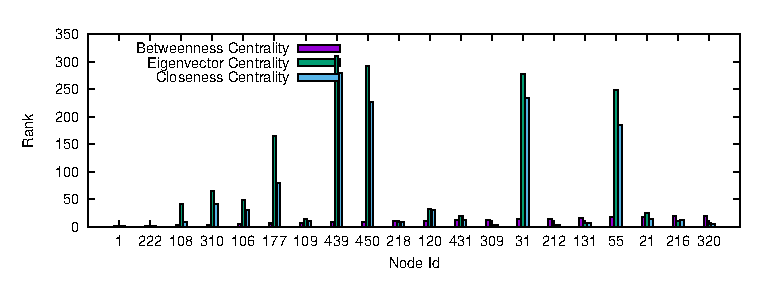
\includegraphics[width=1\textwidth]{figures/social-result_betweenness.eps}
    \caption{Rank comparison for top 20 nodes ranked on betweenness centrality with other centrality scores.}
    \label{fig:social-result-betweenness}
\end{figure*}

\begin{figure*}[!ht]
    \centering
    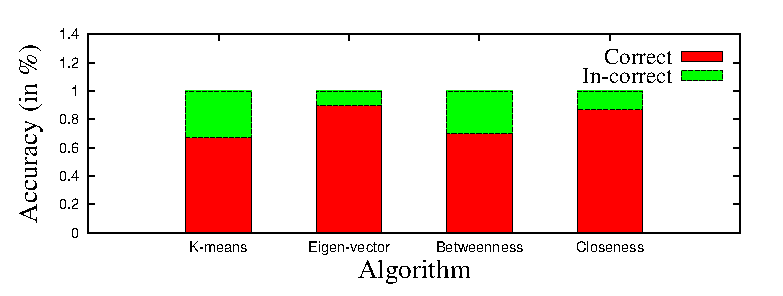
\includegraphics[width=1\textwidth]{figures/social-result_arvind.eps}
    \caption{Comparison of accuracy of algorithms, based on validated result data from Arvind.}
    \label{fig:social-result-arvind}
\end{figure*}

\begin{figure*}[!ht]
    \centering
    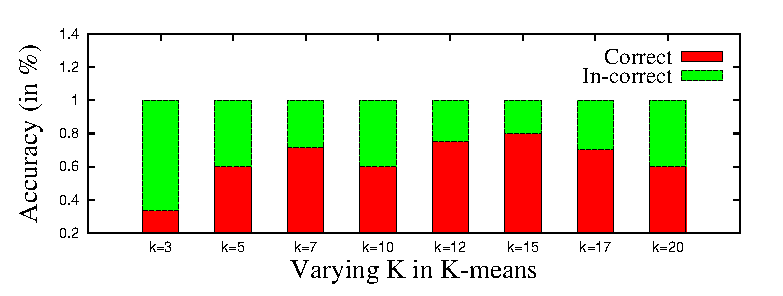
\includegraphics[width=1\textwidth]{figures/social-result_arvind_kmeans.eps}
    \caption{Comparison of accuracy of K-means on varying k, based on validated data from Arvind.}
    \label{fig:social-result-arvind-kmeans}
\end{figure*}

\paragraph{Data Collection}
For our experiments, we have collected Facebook ego network data for
the authors using facebook app "Give me my data"~\cite{givememydata}.
We also called for volunteers to give their data and verify the
results as they know the ground truth data.  For our experiment we
have assigned ids to each user in the data for privacy reasons. 

\paragraph{Results}
We picked assigned each nodes a rank based on the centrality score.
The nodes with higher importance score were ranked accordingly, 1
being the highest rank and $n$ being the lowest rank.  The ego in the
network always gets rank 1.  We then picked top 20 ranked nodes
according to each centrality score, and then compared how much rank
increment or decrement each nodes got in other measures of centrality
scores.

Figure~\ref{fig:social-result-eigen} shows the rank gain or lose for
top 20 nodes for eigenvector centrality scores when compared to other
centrality measures.  Here we can see that node 222, has the same rank
for all the three measures.  So, it shows that a node if it is really
important, remains important irrespective of centrality indicator.  We
can also see that there is not much gain or lose in rank when compared
to closeness centrality.  Node 109 gains a better rank when measured
on different centrality indicators.  But for all other nodes there is
significant drop in rank, when compared to betweenness centrality.

Figure~\ref{fig:social-result-closeness} shows the rank gain or lose for
top 20 nodes for closeness centrality scores when compared to other
centrality measures.  Here we can see that there is significant
overlap in top 20 nodes for closeness centrality and eigenvector
centrality.  Almost 15 nodes out of 20 are common for both the scales.
But when compared to betweenness centrality there is not much overlap.
But still the maximum drop to rank is not more than 45, that is less
than 10\% of the total nodes, 508.  This tells
that nodes that are important according to eigenvector centrality or
closeness centrality measures are really important nodes.  But when we
see the top 20 important nodes for betweenness centrality, see
figure~\ref{fig:social-result-betweenness}, nodes that rank high on
this score, are not among the high ranked nodes on the other
centrality indicators.  Betweenness centrality finds completely
different important nodes.  Some of these nodes are relatively less
important nodes in context of whole network, but these nodes work as a
bridge between two communities in the graph.  That is why these nodes
score high on betweenness centrality but low on other centrality
measures.

%%%%%%%%%%%%%%%%%%%%%%%%%%%%%%%%%%%%%%%%%%%%%%%%%%%%%%%%%%%%%%%%%%%%%%%%%%%%%%
% Table(s) for results of current experiments
%%%%%%%%%%%%%%%%%%%%%%%%%%%%%%%%%%%%%%%%%%%%%%%%%%%%%%%%%%%%%%%%%%%%%%%%%%%%%%

\begin{table*}[th]
\small
\centering
%\begin{tabularx}{\linewidth}{|c|c|c|c|c|c|c|X|}

\begin{tabular}{ c|c|c|c|c|c|c|c|c| }
  \cline{2-9}
  & 
  \multicolumn{2}{c}{\textbf{$u_{1}$}} &
  \multicolumn{2}{|c}{\textbf{$u_{2}$}} &
  \multicolumn{2}{|c}{\textbf{$u_{3}$}} &
  \multicolumn{2}{|c|}{\textbf{root}}  \\
  \cline{2-9}
  \multicolumn{1}{c|}{} &
  with & without & with & without & with & without & with & without\\
  \multicolumn{1}{c|}{} &
  change & changes & changes & changes & changes & changes & changes &
  changes\\
  \hline
  \multicolumn{1}{|c|}{\textbf{create file}}
  & Y & Y & N & Y & N & Y & N & Y \\
  \hline
  \multicolumn{1}{|c|}{\textbf{create dir}}
  & Y & Y & N & Y & N & Y & N & Y \\
  \hline
  \multicolumn{1}{|c|}{\textbf{remove file}}
  & Y & Y & N & Y & N & Y & N & Y \\
  \hline
  \multicolumn{1}{|c|}{\textbf{remove dir}}
  & Y & Y & N & Y & N & Y & N & Y \\
  \hline
  \multicolumn{1}{|c|}{\textbf{create symlink}}
  & Y & Y & N & Y & N & Y & N & Y \\
  \hline
  \multicolumn{1}{|c|}{\textbf{read symlink}}
  & Y & Y & N & Y & N & Y & N & Y \\
  \hline
  \multicolumn{1}{|c|}{\textbf{write symlink}}
  & Y & Y & N & Y & N & Y & N & Y \\
  \hline
  \multicolumn{1}{|c|}{\textbf{create hardlink}}
  & Y & Y & N & Y & N & Y & N & Y \\
  \hline
  \multicolumn{1}{|c|}{\textbf{write hardlink}}
  & Y & Y & N & Y & N & Y & N & Y \\
  \hline
  \multicolumn{1}{|c|}{\textbf{stat}}
  & Y & Y & N & Y & N & Y & N & Y \\
  \hline
  \multicolumn{1}{|c|}{\textbf{change dir}}
  & Y & Y & N & Y & N & Y & N & Y \\
  \hline
  \multicolumn{1}{|c|}{\textbf{read file}}
  & Y & Y & N & Y & N & Y & N & Y \\
  \hline
  \multicolumn{1}{|c|}{\textbf{write file}}
  & Y & Y & N & Y & N & Y & N & Y \\
  \hline
  \multicolumn{1}{|c|}{\textbf{create tar}}
  & Y & Y & N & Y & N & Y & N & Y \\
  \hline
  \multicolumn{1}{|c|}{\textbf{untar}}
  & Y & Y & N & Y & N & Y & N & Y \\
  \hline
  \multicolumn{1}{|c|}{\textbf{make}}
  & Y & Y & N & Y & N & Y & N & Y \\
  \hline
  \multicolumn{1}{|c|}{\textbf{rename}}
  & Y & Y & N & Y & N & Y & N & Y \\
  \hline
\end{tabular}

%\end{tabularx}
\caption{\capfont Results of different file system operations for
different users, with and without the changes.}
\label{tab:results}
\end{table*}

%%%%%%%%%%%%%%%%%%%%%%%%%%%%%%%%%%%%%%%%%%%%%%%%%%%%%%%%%%%%%%%%%%%%%%%%%%%%%%
%% For Emacs:
% Local variables:
% fill-column: 70
% End:
%%%%%%%%%%%%%%%%%%%%%%%%%%%%%%%%%%%%%%%%%%%%%%%%%%%%%%%%%%%%%%%%%%%%%%%%%%%%%%
%% For Vim:
% vim:textwidth=70
%%%%%%%%%%%%%%%%%%%%%%%%%%%%%%%%%%%%%%%%%%%%%%%%%%%%%%%%%%%%%%%%%%%%%%%%%%%%%%
% LocalWords:  PEAFS PEAIO Lustre SBU HMC config


\paragraph{Result validation}
We run the experiments on \emph{4} different ego networks collected
from volunteers.  To verify the experimental results with the ground
truth data, we send the top 30 nodes to the users to verify how many
of them are actually important.  Their reponse is treated as
\emph{verified ground truth} and is used to compare the efficiency of
algorithms.

We also had run k-means clustering algorithm on the ego network for
different k values.  For k-means clustering we have used shortest path
distance between two nodes after excluding the ego from the graph as a
distance metric.  After clustering the graph, we report centroid of
each group as important nodes.  Table~\ref{tab:k-means-results} shows
the important nodes that were reported for k=5 and their rank
according to different centrality measures.   We have varied the
number of clusters for $k=3,5,7,10,12,15,17,20$ and compared the
reported nodes with the ground truth data in
Figure~\ref{fig:social-result-arvind-kmeans}.  We observed that kmeans
works best for k=15 and worst for k=3.  An ego-network of 3 cluster is not
very practical scenario, so its results are not accurate.  Accuracy of
kmeans is more than \emph{60\%} for all other cases.

\paragraph{Accuracy of algorithms}
We compare the experimental results with the verified grund truth
and find the accuracy of an algorithm in terms of \% match.  In
Figure~\ref{fig:social-result-arvind} we compared the results from ego
network of \emph{Arvind} with the ground truth data.  In this we have
taken mean accuracy of k-means along with accuracy of others. It shows
that closeness and eigen-vector give similar results.  We have also
compared the verified ground truth data for all the users in
Table~\ref{tab:accuracy-of-algorithms}.  We observe that eigen-vector
centrality gives the most accurate results and it is consistent across
all ego networks.

%%%%%%%%%%%%%%%%%%%%%%%%%%%%%%%%%%%%%%%%%%%%%%%%%%%%%%%%%%%%%%%%%%%%%%%%%%%%%%
%% For Emacs:
% Local variables:
% fill-column: 70
% End:
%%%%%%%%%%%%%%%%%%%%%%%%%%%%%%%%%%%%%%%%%%%%%%%%%%%%%%%%%%%%%%%%%%%%%%%%%%%%%%
%% For Vim:
% vim:textwidth=70
%%%%%%%%%%%%%%%%%%%%%%%%%%%%%%%%%%%%%%%%%%%%%%%%%%%%%%%%%%%%%%%%%%%%%%%%%%%%%%
% LocalWords:

%\section{Related Work}
\label{related}

%Related work section...
%
%Typical length: 0.5-2.0 papers, avg 1.0 (assuming a 12-14
%conf. paper).
%
%Background and Related Work can be similar.
%Most citations will be in this section.
%
%Describe past work and criticize it, fairly.  Use citations to
%JUSTIFY your criticism! Now you can fairly compare to YOUR work.
%
%Problem: don't put background/motivation material here (too
%late).
%
%Important: when it doubt, cite it! (to avoid not citing a
%reviewer's own papers, or papers they know or "think" are
%related).
%
%If conf. allows unlimited citations, do so.
%
%Organize past work: should it be importance order?
%chronological? categorical?

File based encryption are popular and have been deployed widely.  Matt
Blaze designed Cryptographic File System (CFS) pushes encryption
services into the file system itself~\cite{cfs}.  CFS supports secure
storage at the system level through a standard Unix file system
interface to encrypted files.  Users associate a cryptographic key
with the directories they wish to protect.  Files in these directories
(as well as their pathname components) are transparently encrypted and
decrypted with the specified key without further user intervention;
plain text is never stored on a disk or sent to a remote file server.
CFS can use any available file system for its underlying storage
without modification, including remote file servers such as NFS.
System management functions, such as file backup, work in a normal
manner and without knowledge of the key.

EncFS is a user-space stackable cryptographic file-system similar to
eCryptfs, and aims to secure data with the minimum
hassle~\cite{encfs}.  It uses FUSE to mount an encrypted directory
onto another directory specified by the user.  It does not use a
loopback system like some other comparable systems such as TrueCrypt
and dm-crypt.

Existing cryptographic file systems for Unix do not take into account
that sensitive data must often be shared with other users, but still
kept secret.  By design, the only one who has access to the secret
data is the person who encrypted it and therefore knows the encryption
key or password.  This paper presents a kernel driver for a new
encrypted file system, called Fairly Secure File System (FSFS), which
provides mechanisms for user management and access control for
encrypted files~\cite{fsfs}.  The driver has been specifically
designed with multi user systems in mind.  FSFS also tries to prevent
unintentional transfer of sensitive data to unencrypted file systems,
where it would be stored in plain text.


%%%%%%%%%%%%%%%%%%%%%%%%%%%%%%%%%%%%%%%%%%%%%%%%%%%%%%%%%%%%%%%%%%%%%%%%%%%%%%
%% For Emacs:
% Local variables:
% fill-column: 70
% End:
%%%%%%%%%%%%%%%%%%%%%%%%%%%%%%%%%%%%%%%%%%%%%%%%%%%%%%%%%%%%%%%%%%%%%%%%%%%%%%
%% For Vim:
% vim:textwidth=70
%%%%%%%%%%%%%%%%%%%%%%%%%%%%%%%%%%%%%%%%%%%%%%%%%%%%%%%%%%%%%%%%%%%%%%%%%%%%%%
% LocalWords:  SMR HDDs drive's SMRs

\section{Conclusions}
\label{conc}

%Conclusion text...
%
%Length: 0.25-0.5 pages max (1-2 pgfs)
%
%Summary of key contributions (should match your design goals).
%Not summary of whole paper.  Any novel contributions mentioned.
%Summarize good eval results.
%
%Key: give reader the "take home" message.

We found important nodes in an ego network using different centrality
measures.  Also we found the important nodes by dividing the ego
network using k-means clustering and reporting the centroid as the
important node.  We see that eigenvector centrality is the most
accurate measure of the identifying the important nodes.  Closeness
centrality also performs well as compared to betweenness centrality.
We also see that k-means clustering also identifies the important node
when number of communities are more than 5.  We can conclude that some
nodes are more important than other for one measure, but less
important for different measure.  There are nodes also, that are
important for all kind of measures of importance.

\paragraph{Future Work}
We plan to extend k-means clustering algorithm by not reporting the
centroid of the cluster as important node.  We'll run eigenvector
centrality algorithm on each cluster and then report the important
nodes.  We'll also try to improve the betweenness centrality as
current betweenness centrality algorithm is not applicable to
disconnected graphs.  And presence of ego affects the outcome of the
algorithm severely most of the shortest paths will pass through ego,
and the distance can not be more than 2.

%Future work text...
%
%Typical length: 0.25-0.33 pages max
%
%Don't write too much:
%- the more you write, the more work appears "premature"
%- takes up important space (small impact on acceptance)
%
%Often folded as subsection of conclusions.
%
%Describe most important 1-3 "novel/research" future work ideas.
%
%Avoid "short term" future goals.  Focus on long-term goals, well
%beyond the scope of THIS paper.  Avoid stuff that might be
%considered as should have been part of this work.
%
%Give reader some ideas of HOW you plan to go about investigating
%future ideas.
%

%%%%%%%%%%%%%%%%%%%%%%%%%%%%%%%%%%%%%%%%%%%%%%%%%%%%%%%%%%%%%%%%%%%%%%%%%%%%%%
%% For Emacs:
% Local variables:
% fill-column: 70
% End:
%%%%%%%%%%%%%%%%%%%%%%%%%%%%%%%%%%%%%%%%%%%%%%%%%%%%%%%%%%%%%%%%%%%%%%%%%%%%%%
%% For Vim:
% vim:textwidth=70
%%%%%%%%%%%%%%%%%%%%%%%%%%%%%%%%%%%%%%%%%%%%%%%%%%%%%%%%%%%%%%%%%%%%%%%%%%%%%%
% LocalWords:

\paragraph{Acknowledgments}
\label{ack}

%1 pgf max.
%
%Optional if you have space.  Cannot ack in anonymous
%submissions.
%
%List anyone who helped ideas, review drafts, but isn't a
%co-author.
%
%List any funding agency that supported the work (some agencies
%require this).
%
%Example:
%
%We thank the EMC/Data Domain performance team for their help.  We also
%thank Windsor Hsu, our shepherd Jiri Schindler and our anonymous
%reviewers for their helpful feedback.  This work was supported in part
%by NSF award CCF-0937854.

We thank Professor Erez Zadok for guidance and rigorous design reviews.
We also thank Ming Chen for helping with the \emph{XFSTESTS}.

%%%%%%%%%%%%%%%%%%%%%%%%%%%%%%%%%%%%%%%%%%%%%%%%%%%%%%%%%%%%%%%%%%%%%%%%%%%%%%
%% For Emacs:
% Local variables:
% fill-column: 70
% End:
%%%%%%%%%%%%%%%%%%%%%%%%%%%%%%%%%%%%%%%%%%%%%%%%%%%%%%%%%%%%%%%%%%%%%%%%%%%%%%
%% For Vim:
% vim:textwidth=70
%%%%%%%%%%%%%%%%%%%%%%%%%%%%%%%%%%%%%%%%%%%%%%%%%%%%%%%%%%%%%%%%%%%%%%%%%%%%%%
% LocalWords:  SMR HDDs drive's SMRs

%\clearpage

%\appendix
%\section{General Purpose Notes}

\subsection{Notes About Picking a Project}

Put every possible related citation you can! (esp. if conf.
doesn't count citations towards page size).

Literature survey:
- CiteSeer

- Google Scholar

- libraries

1. find a few relates paper

2. skim papers to find relevance

3. search for add'l related papers in Biblio.

4. reverse citation: use srch engines, to find
   newer papers that cite the paper you like.

5. "stop" when reach transitive closure

- then go off and read it; summarize papers

- think about "how can I improve" and "what was so
  good about that paper".

- check future work for project ideas.

- go to talks \& conferences

Pick an idea:

- novelty vs. incremental (how big of an increment?)

- idea vs. practical implications
  (implemented? released? in use as OSS or commercial?)

- where to submit? good fit and match for quality.

- look at schedule of conferences: due dates \& result dates.
i.e., what's the due dates, when do you hear an accept/reject
notice by; if the paper is rejected, where/when can you submit
it to next?

\subsection{Different Types of Technical Papers}

Computer systems field:

- operating systems, networking, security

- programming, virtualization, storage

- architecture, databases, etc.

- NOT: theory

1. conference paper: mature, completed work. [length 6-14 pages]

2. workshop paper: short, work-in-progress report [4-6 pp]

- special workshop type: a "position" paper, often called "Hot-???"

3. journal article: expanded version of a conference/workshop
   paper.  No page limit.  Common to follow up a workshop and even
   a conf. paper with an exapnded journal version. Journals often
   ask for at least 25\% more "new" material.

Conf./workshop/journals are "refereed" publications, meaning that
your peers get to review the document and accept/reject it, and
return comments to you.  Non-refereed pubs are usually called
"technical reports": anyone can publish a TR on their own.

Workshop and conf. papers get presented in person: usually lead
author would give the talk.  Journals are not presented.

In this class, you will submit a "position" paper (your design
document, 2 pp); by end of term, you'll submit a longer conf. like'
paper (6+ pp).

Conf./workshop papers review cycle: 1-4 months

- journals: no time limit; often; no deadline often 6+ months.

Conf./workshop papers get an accept/reject notice:

- rate: a conditional accept pending "shepherd's aproval"

Journals: phases of aproval:

- reject: "go away"

- major revision: a reject; ask to make major changes and resubmit.

- minor revision: a reject; ask to make minor changes and resubmit.

- conditional accept: very minor changes asked (usually prose,
  typos, English)

- accept: manuscript is accepted as is.

Publishing cycles, from moment of receiving an "accept notice":

- workshop/conf.: 2-3 months; present @ venue 2-3 months later.

- journal: 2-6 months

A manuscript is considered published on 1st day of workshop/conf.
or the first day of the month in which the journal is published.

%%%%%%%%%%%%%%%%%%%%%%%%%%%%%%%%%%%%%%%%%%%%%%%%%%%%%%%%%%%%%%%%%%%%%%%%%%%%%%
%% For Emacs:
% Local variables:
% fill-column: 70
% End:
%%%%%%%%%%%%%%%%%%%%%%%%%%%%%%%%%%%%%%%%%%%%%%%%%%%%%%%%%%%%%%%%%%%%%%%%%%%%%%
%% For Vim:
% vim:textwidth=70
%%%%%%%%%%%%%%%%%%%%%%%%%%%%%%%%%%%%%%%%%%%%%%%%%%%%%%%%%%%%%%%%%%%%%%%%%%%%%%
% LocalWords:  SMR HDDs drive's SMRs




\bibliographystyle{plain}
\bibliography{template/master,smr}
%{\footnotesize \bibliography{template/master}}

%\newpage

\end{document}

%%%%%%%%%%%%%%%%%%%%%%%%%%%%%%%%%%%%%%%%%%%%%%%%%%%%%%%%%%%%%%%%%%%%%%%%%%%%%%
%% For Emacs:
% Local variables:
% fill-column: 70
% End:
%%%%%%%%%%%%%%%%%%%%%%%%%%%%%%%%%%%%%%%%%%%%%%%%%%%%%%%%%%%%%%%%%%%%%%%%%%%%%%
%% For vim:
% vim:textwidth=70
%%%%%%%%%%%%%%%%%%%%%%%%%%%%%%%%%%%%%%%%%%%%%%%%%%%%%%%%%%%%%%%%%%%%%%%%%%%%%%
% LocalWords:

% LocalWords:  Ankur Agrawal Benixon Arul Dhas Hospodor Yangwook Kang Rekha UC
% LocalWords:  Pitchumani Sphurti Sortur USletter csrg smr
